
\subsection{Problem Statement}

\begin{frame}{Introduction}
    \begin{itemize}
        \item Overview condensed matter physics
              %   \only<1>{    \begin{itemize}
              %           \item a \todo{test}
              %       \end{itemize} }
              \only<2->{ \item Strongly correlated materials } \only<2>{ \cite{Alexandradinata2020}
                  \begin{itemize}
                      \item Superconductors
                      \item Quantum  spin  liquids
                      \item Strange metals
                      \item Quantum Criticality
                      \item Correlated topological matter
                  \end{itemize}
              }
              \only<3->{ \item How to proceed }
              \only<3>{
                  \begin{itemize}
                      \item Material synthesis and discovery
                      \item Numerical methods
                      \item Analytical methods
                  \end{itemize}
              }
    \end{itemize}
\end{frame}

\begin{frame}{Simulating Quantum Many-body Systems}
    \begin{itemize}
        \item Equations are known
        \item Curse of dimensionality
        \item Tensor networks
    \end{itemize}
\end{frame}

\subsection{Tensor Networks}

\begin{frame}{Tensor Networks: Introduction}

    \begin{equation}
        \ket{\Psi} = \sum_{i_1 i_2 \cdots i_n } C^{i_1 i_2 \cdots i_n} \ket{i_1} \otimes \ket{i_2} \otimes \cdots \otimes \ket{i_n}.
    \end{equation}
    \begin{equation} \label{c_split}
        C^{i_1 i_2 \cdots i_n} = Tr( C^{i_1} C^{i_2} \cdots C^{i_n} M  ).
    \end{equation}

\end{frame}

\begin{frame}{Tensor Networks: Graphical Notation}
    \begin{table}[]
        \centering
        \begin{tabular}{l|l|l}
            conventional            & Einstein                & tensor notation           \\
            \hline
            $\Vec{x}$               & $x_{\alpha}$            &

            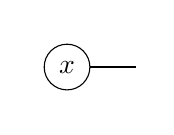
\begin{tikzpicture}[baseline=({N2.base}) ]
                \clip (-0.5,-0.5) rectangle (1,0.5);
                \node[circle, draw] (N2) at (0,0) {$x$};
                \node[] (N1) at (1,0) {};
                \draw  (N1) -- (N2) ;
            \end{tikzpicture}                                                     \\
            M                       & $M_{\alpha \beta}$      & 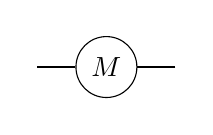
\begin{tikzpicture}[baseline={0cm-0.5*height("$=$")} ]
                \clip (-1,-0.5) rectangle (1,0.5);

                \node[circle, draw] (N2) at (0,0) {$M$};
                \node[] (N0) at (-1,0) {};
                \node[] (N1) at (1,0) {};

                \draw  (N1) -- (N2) ;
                \draw  (N0) -- (N2) ;

            \end{tikzpicture} \\

            $\Vec{x} \cdot \Vec{y}$ & $x_{\alpha} y_{\alpha}$ & 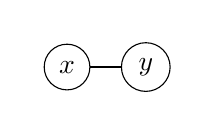
\begin{tikzpicture}[baseline=({N2.base}) ]
                \clip (-0.5,-0.5) rectangle (1.5,0.5);
                \node[circle, draw] (N2) at (0,0) {$x$};
                \node[circle, draw] (N1) at (1,0) {$y$};
                \draw  (N1) -- (N2) ;
            \end{tikzpicture} \\
        \end{tabular}
    \end{table}
\end{frame}

\def \mpograph {\mpo{5}{{"Tr","$\chi$",,,,}}{{"$i_1$","$i_2$",,"$i_n$","-"}}{{"-","-",,"-","-"}}{{0,0,1,0,0}}{{"C", "C",,"C","M" }}}

\def \ctens { \begin{tikzpicture}[baseline={0.5cm-0.5*height("$=$")}]

        \draw (-3,-0) rectangle (1,1)  [add reference=C]   ;
        \node  at (C center) {C};

        \node (N1)  at  (-2.5,1.6) {$i_1$};
        \node (N2)  at  (-1.5,1.6) {$i_2$};
        \node  at  (-.5,1.25) {...};
        \node  (N3) at  (.5,1.6) {$i_n$};

        \draw    (N1) -- (N1 |-  C north);
        \draw    (N2) -- (N2 |-  C north);
        \draw    (N3) -- (N3 |-  C north);

    \end{tikzpicture} }

\begin{frame}

    \begin{equation}
        C^{i_1 i_2 \cdots i_n} = Tr( C^{i_1} C^{i_2} \cdots C^{i_n} M )
    \end{equation}
    \begin{equation}
        \ctens  \; = \mpograph
    \end{equation}
\end{frame}

\begin{frame}{Tensor Networks: Operators}

    \begin{equation}
        \hat{O} =   \vcenter{\hbox{ \pepob{5}{3}{{
                            "-","-", "-","-",
                            "","","","",
                            "-","-", "-","-",}}{{
                            "-","-",
                            "","",
                            "","",
                            "","",
                            "-","-",}}{{
                            4,4,4,4,4,
                            13,0,0,0,13,
                            4,4,4,4,4,}} }}
    \end{equation}

    \begin{equation}
        \hat{O} \ket{\Psi} =  \vcenter{\hbox{ \pepob{5}{3}{{
                            "-","-", "-","-",
                            "","$\chi$","","",
                            "","$\chi$","","",}}{{
                            "-", "-",
                            "", "",
                            "", "",
                            "", "",
                            "-", "-",}}{{
                            4,4,4,4,4,
                            13,0,0,0,13,
                            13,0,0,0,13}}  }} =   \vcenter{\hbox{ \pepob{5}{2}{{
                            "-","-", "-","-",
                            "","$\chi^2$","",""}}{{
                            "-",
                            "",
                            "",
                            "",
                            "-"}}{{
                            4,4,4,4,4,
                            13,0,0,0,13}} }}
    \end{equation}

\end{frame}

\subsection{Overview Thesis}

\begin{frame}{Operator exponential}
    \begin{itemize}
        \item (Real) Time eveolution: $\hat{O} = e^{ - i \hat{H} t }  $
        \item Statistical ensembles: $\hat{O} = e^{ - \beta \hat{H}   }$
    \end{itemize}
\end{frame}

